%%
%% Copyright 2007, 2008, 2009 Elsevier Ltd
%%
%% This file is part of the 'Elsarticle Bundle'.
%% ---------------------------------------------
%%
%% It may be distributed under the conditions of the LaTeX Project Public
%% License, either version 1.2 of this license or (at your option) any
%% later version.  The latest version of this license is in
%%    http://www.latex-project.org/lppl.txt
%% and version 1.2 or later is part of all distributions of LaTeX
%% version 1999/12/01 or later.
%%
%% The list of all files belonging to the 'Elsarticle Bundle' is
%% given in the file `manifest.txt'.
%%

%% Template article for Elsevier's document class `elsarticle'
%% with numbered style bibliographic references
%% SP 2008/03/01
%%
%%
%%
%% $Id: elsarticle-template-num.tex 4 2009-10-24 08:22:58Z rishi $
%%
%%
\documentclass[preprint,12pt]{elsarticle}

%% Use the option review to obtain double line spacing
%% \documentclass[preprint,review,12pt]{elsarticle}

%% Use the options 1p,twocolumn; 3p; 3p,twocolumn; 5p; or 5p,twocolumn
%% for a journal layout:
%% \documentclass[final,1p,times]{elsarticle}
%% \documentclass[final,1p,times,twocolumn]{elsarticle}
%% \documentclass[final,3p,times]{elsarticle}
%% \documentclass[final,3p,times,twocolumn]{elsarticle}
%% \documentclass[final,5p,times]{elsarticle}
%% \documentclass[final,5p,times,twocolumn]{elsarticle}

%% if you use PostScript figures in your article
%% use the graphics package for simple commands
%% \usepackage{graphics}
%% or use the graphicx package for more complicated commands
%% \usepackage{graphicx}
%% or use the epsfig package if you prefer to use the old commands
%% \usepackage{epsfig}

%% The amssymb package provides various useful mathematical symbols
\usepackage{amssymb}
%% The amsthm package provides extended theorem environments
%% \usepackage{amsthm}

%\usepackage{multirow}
\usepackage{rotating}
\usepackage{epsfig}
\usepackage[centertags]{amsmath}

%% The lineno packages adds line numbers. Start line numbering with
%% \begin{linenumbers}, end it with \end{linenumbers}. Or switch it on
%% for the whole article with \linenumbers after \end{frontmatter}.
%% \usepackage{lineno}

%% natbib.sty is loaded by default. However, natbib options can be
%% provided with \biboptions{...} command. Following options are
%% valid:

%%   round  -  round parentheses are used (default)
%%   square -  square brackets are used   [option]
%%   curly  -  curly braces are used      {option}
%%   angle  -  angle brackets are used    <option>
%%   semicolon  -  multiple citations separated by semi-colon
%%   colon  - same as semicolon, an earlier confusion
%%   comma  -  separated by comma
%%   numbers-  selects numerical citations
%%   super  -  numerical citations as superscripts
%%   sort   -  sorts multiple citations according to order in ref. list
%%   sort&compress   -  like sort, but also compresses numerical citations
%%   compress - compresses without sorting
%%
%% \biboptions{comma,round}

% \biboptions{}


\journal{JSS}

\begin{document}

\begin{frontmatter}

%% Title, authors and addresses

%% use the tnoteref command within \title for footnotes;
%% use the tnotetext command for the associated footnote;
%% use the fnref command within \author or \address for footnotes;
%% use the fntext command for the associated footnote;
%% use the corref command within \author for corresponding author footnotes;
%% use the cortext command for the associated footnote;
%% use the ead command for the email address,
%% and the form \ead[url] for the home page:
%%
%% \title{Title\tnoteref{label1}}
%% \tnotetext[label1]{}
%% \author{Name\corref{cor1}\fnref{label2}}
%% \ead{email address}
%% \ead[url]{home page}
%% \fntext[label2]{}
%% \cortext[cor1]{}
%% \address{Address\fnref{label3}}
%% \fntext[label3]{}


\title{A Multi-objective Approach to FSS in Software Quality}

%% use optional labels to link authors explicitly to addresses:
%% \author[label1,label2]{<author name>}
%% \address[label1]{<address>}
%% \address[label2]{<address>}

\author[uah,ob]{D. Rodr\'iguez\corref{cor1}}
\ead{daniel.rodriguezg@uah.es}

%\author[ob]{R. Harrison}
%\ead{rachel.harrison@brookes.ac.uk}

\cortext[cor1]{Corresponding author.}
\address[uah]{Department of Computer Science, University of Alcal\'a, Ctra. Barcelona, Km. 31.6, 28871 Alcal\'a de Henares, Madrid, Spain}

\address[ob]{School of Technology, Oxford Brookes University\\ Wheatley Campus, Oxford OX33 1HX, UK}

\begin{abstract}

%
%\begin{itemize}
%  \item Background:
%  \item Aim:
%
%  \item Method:
%
%  \item Results:
%
%  \item Conclusions: %
%\end{itemize}
%
\end{abstract}

\begin{keyword}
%% keywords here, in the form: keyword \sep keyword

%% MSC codes here, in the form: \MSC code \sep code
%% or \MSC[2008] code \sep code (2000 is the default)

FSS \sep Multi-objective \sep  datasets \sep ISBSG repository

\end{keyword}

\end{frontmatter}

%%
%% Start line numbering here if you want
%%
% \linenumbers

%%%%%%%%%%%%%%%%%%%%%%%%%%%%%%%%%%%%%%%%%%%%%%%%%%%%%%%%%%%%%%%%%%%%%
%%%%%%%%%%%%%%%%%%%%%%%%%%%%%%%%%%%%%%%%%%%%%%%%%%%% Introduction %%%
%%%%%%%%%%%%%%%%%%%%%%%%%%%%%%%%%%%%%%%%%%%%%%%%%%%%%%%%%%%%%%%%%%%%%

\section{Introduction}
\label{sec:introduction}

FSS very important

Multi-ojbective too

Objectives

Stability + Accuracy


\begin{figure}
 \centering
 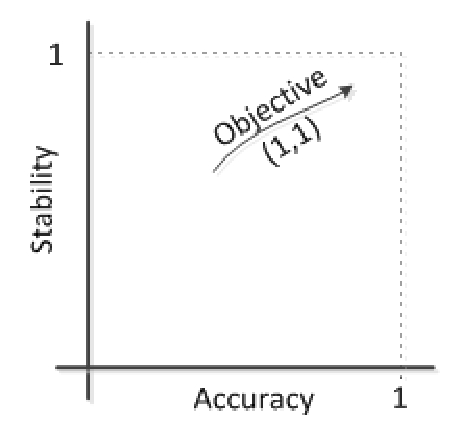
\includegraphics[width=.45\columnwidth]{./figs/objective.eps}
 % Classification.eps: 0x0 pixel, 300dpi, 0.00x0.00 cm, bb=14 14 225 190
 \caption{Stability vs. Accuracy}
 \label{fig:stabilityVsAcc}
\end{figure}

%%%%%%%%%%%%%%%%%%%%%%%%%%%%%%%%%%%%%%%%%%%%%%%%%%%%%%%%%%%%%%%%%%%%%%%%%%%%%
%%%%%%%%%%%%%%%%%%%%%%%%%%%%%%%%%%%%%%%%%%%%%%%%%%%%%%%%%%%% Related Work %%%
%%%%%%%%%%%%%%%%%%%%%%%%%%%%%%%%%%%%%%%%%%%%%%%%%%%%%%%%%%%%%%%%%%%%%%%%%%%%%
\section{Related Work}
\label{sec:relatedWork}

FSS

Stability

Consistency index [15] is used to measure the degree of similarity between the metric rankings of two feature selection techniques.

The consistency index takes into consideration bias due to chance. We compute the consistency index
between two feature subsets as follows. Let $T_i$ and $T_j$ be subsets of features, where $|Ti| = |Tj | = k$. The consistency index [15] is obtained as follows:

\begin{equation}\label{eq:CI}
    I_C (T_i, T_j ) = frac{dn-k^2}{k(n-k)}
\end{equation}



where $n$ is the total number of features in the dataset, $d$ is the
cardinality of the intersection between subsets $T_i$ and $T_j$ , and
$-1 < IC (Ti, Tj) < 1$. The greater the consistency index, the
more similar the subsets are. If the two rankings are the same, then $I_C=1$.

If there is no overlap between two rankings, then the consistency
index is -0.1667???

We consider two algorithms to be similar if they share 2/3 out of the top features.

%L. I. Kuncheva, �A stability index for feature selection,� in Proceedings
%of the 25th conference on Proceedings of the 25th IASTED International
%Multi-Conference: artificial intelligence and applications. Anaheim,
%CA, USA: ACTA Press, 2007, pp. 390�395.


M. Hall, G. Holmes, Benchmarking Attribute Selection Techniques for
Discrete Class Data Mining, IEEE Trans. on Knowledge and Data En-
gineering 15 (6) (2003) 1437-1447.

Y. Yang, J. O. Pedersen, A Comparative Study on Feature Selection in
Text Categorization, in: Proc. 14th Intl. Conf. on Machine Learning,
Morgan Kaufmann Publishers Inc., San Francisco, CA, USA, 1997, pp.
412-420

%%%%%%%%%%%%%%%%%%%%%%%%%%%%%%%%%%%%%%%%%%%%%%%%%%%%%%%%%%%%%%%%%%%%%
%%%%%%%%%%%%%%%%%%%%%%%%%%%%%%%%%%%%%%%%%%%%% Threats to Validity %%%
%%%%%%%%%%%%%%%%%%%%%%%%%%%%%%%%%%%%%%%%%%%%%%%%%%%%%%%%%%%%%%%%%%%%%

%\section{Threats to Validity}
%\label{sec:threats}
%
%As with all empirical studies, there are some threats to validity that need to be considered in this study.

%\emph{Construct validity} is the degree to which the variables used in the study accurately measure the concepts they are supposed to measure. We have only used those projects classified with the quality attribute classified as A or B. Although there seems to be an agreement about the practical usefulness of publicly available repositories and a large amount of work using such datasets, the origin of the data is not completely known and therefore such a risk is present. There is also a risk in the way that the preprocessing of the dataset was performed (e.g., considering that all versions of Visual Basic are equivalent, unifying the consistency across the languages and their generation type, etc).
%
%\emph{Internal validity} is the degree to which conclusions can be drawn. A major threat can be related to the preprocessing performed. Although we have reported and specified each step, we may have discarded relevant attributes or joined values incorrectly. We also needed to deal with a large number of missing values for some of the attributes. For example, after the preprocessing, the maximum team size and average time size variables have almost 60\% and 80\% of missing values respectively with the risk of being very few or even a single organisation reporting such attributes. It could have been very valuable to know which projects correspond to a particular company, and other measures about personnel stability. The ISBSG does not report detailed information about the personnel characteristics and it is known that there are large differences in productivity. Therefore, projects of similar size can differ hugely in the amount of time and effort required. We are not able to analyse such characteristics with this repository. We believe that their usefulness is not clearly proven for some data mining and statistical analyses.
%
%\emph{External validity} is the degree to which the results of the research can be generalised to the population under study and other research settings. Although the data comes from real projects and is in principle, generalisable, the ISBSG organisation recognise these project may not be representative of the industry (they are selected by the companies providing the data which in turn belong to the better performed organisations with experience  using function point estimation techniques). In the context of estimation, Kitchenham et al.~\cite{Kitchenham:2007} performed a Systematic Literature Review of predictions from cross-company models with predictions from within-company models. Although the authors state that their results are inconclusive as there is support in both directions, it seems to be easy to misuse cross-company models. In any case, each organisation should select and perform the studies and estimations with subsets of the data close to their domain and organisation type, environment, language, etc.


%%%%%%%%%%%%%%%%%%%%%%%%%%%%%%%%%%%%%%%%%%%%%%%%%%%%%%%%%%%%%%%%%%%%%
%%%%%%%%%%%%%%%%%%%%%%%%%%%%%%%%%%%%%%%%%%%%%%%%%%%%%% Conclusion %%%
%%%%%%%%%%%%%%%%%%%%%%%%%%%%%%%%%%%%%%%%%%%%%%%%%%%%%%%%%%%%%%%%%%%%%

\section{Conclusions and Future Research Directions}
\label{sec:conclusions}

In this paper, we analysed

In future work, further statistical and data mining studies will be performed with the ISBSG repository as well as other repositories in order to study the quality of such repositories, validate generic claims found in the literature and provide guidelines for decision making.


%%%%%%%%%%%%%%%%%%%%%%%%%%%%%%%%%%%%%%%%%%%%%%%%%%%%%%%%%%%%%%%%%%%%%
%%%%%%%%%%%%%%%%%%%%%%%%%%%%%%%%%%%%%%%%%%%%%%%%%%% ACKNOLEDGEMENT %%
%%%%%%%%%%%%%%%%%%%%%%%%%%%%%%%%%%%%%%%%%%%%%%%%%%%%%%%%%%%%%%%%%%%%%
%\section*{Acknowledgment}
%
%This research was supported by ...


%% The Appendices part is started with the command \appendix;
%% appendix sections are then done as normal sections
%% \appendix

%% \section{}
%% \label{}

%% References
%%
%% Following citation commands can be used in the body text:
%% Usage of \cite is as follows:
%%   \cite{key}         ==>>  [#]
%%   \cite[chap. 2]{key} ==>> [#, chap. 2]
%%

%% References with bibTeX database:

%%%%%%%%%%%%%%%%%%%%%%%%%%%%%%%%%%%%%%%%%%%%%%%%%%%%%%%%%%%%%%%%%%%%%%%%%%%%%
%%%%%%%%%%%%%%%%%%%%%%%%%%%%%%%%%%%%%%%%%%%%%%%%%%%%%%%%%%%%%% References %%%
%%%%%%%%%%%%%%%%%%%%%%%%%%%%%%%%%%%%%%%%%%%%%%%%%%%%%%%%%%%%%%%%%%%%%%%%%%%%%

\bibliographystyle{model1b-num-names}
\bibliography{./refs/references}

%% Authors are advised to submit their bibtex database files. They are
%% requested to list a bibtex style file in the manuscript if they do
%% not want to use elsarticle-num.bst.

%% References without bibTeX database:

% \begin{thebibliography}{00}

%% \bibitem must have the following form:
%%   \bibitem{key}...
%%

% \bibitem{}

% \end{thebibliography}

%%%%%%%%%%%%%%%%%%%%%%%%%%%%%%%%%%%%%%%%%%%%%%%%%%%%%%%%%%%%%%%%%%%%%%%%%%%%%
%%%%%%%%%%%%%%%%%%%%%%%%%%%%%%%%%%%%%%%%%%%%%%%%%%%%%%%%%%%%%%%% Appendix %%%
%%%%%%%%%%%%%%%%%%%%%%%%%%%%%%%%%%%%%%%%%%%%%%%%%%%%%%%%%%%%%%%%%%%%%%%%%%%%%

% \appendix
% \label{app:ISGSGAttrbutes}
%
% \section{ISBSG Attributes Used in this Study}


\end{document}

%%
%% End of file `elsarticle-template-num.tex'.
